
\documentclass[openany]{book} % openany allows chapters to start on either an odd or an even page

\usepackage[top=1in, bottom=1in, left=1in, right=1in]{geometry}
\usepackage{parskip}  % Disables indentation at paragraph breaks
\usepackage{amsmath, amssymb}  % Math symbols, etc.
\usepackage{physics}  % A ton of physics macros and other useful things
\usepackage{graphicx}

\usepackage{matlab-prettifier}


\newcommand{\minimize}[1]{\underset{#1}{\textrm{minimize}} \, }

% The notation Ng uses for indexing is a pain to typeset
\renewcommand{\ss}[2]{_{#1}^{(#2)}}
\newcommand{\s}[1]{\ss{}{#1}}

\newcommand{\xij}{x\ss{j}{i}}
\renewcommand{\xi}{x\s{i}} % I will not be using the letter xi
\newcommand{\yi}{y\s{i}}

\newcommand{\hth}{h_\theta}
\newcommand{\hTh}{h_\Theta}

\newcommand{\R}{\mathbb{R}}

\renewcommand{\norm}[1]{\left\lVert #1 \right\rVert}

% Elementwise multiplication
\newcommand{\ewise}{\odot}

% SVM Cost function
\DeclareMathOperator{\cost}{cost}



\title{ \huge{Machine Learning} \\ \vspace{1em} \normalsize{Notes from the Course by Stanford University's Andrew Ng} }
\author{Joshua Brown}
\date{}

\begin{document}

\maketitle
\tableofcontents

\chapter{Week 1}

\section{Model and Cost Functions}

\subsection{Notation}

Some notation will be somewhat unique for this course, and some will be unique just to my notes

\begin{center}
  \begin{tabular}{l l}
    \hline
    Notation                    & Meaning \\
    \hline
    $X$                         & The space of input variables \\
    $\xi$                       & The $i^{th}$ value of an input variable \\
    $Y$                         & The space of outputs \\
    $\yi$                       & The $i^{th}$ value of the output variable \\
    $\theta_j$                  & The $j^{th}$ model parameter \\
    $J(\theta_0, \theta_1)$     & The cost function \\
    $h_{\theta_0, \theta_1}(x)$ & The hypothesis function \\
    \hline
  \end{tabular}
\end{center}

\subsection{Cost Function}

Common cost function ``Mean squared error''

\[  J(\theta_0, \theta_1) = \frac{1}{2m} \sum_{i=1}^m \qty(\hat{y}_i - y_i)^2 \]

\[  J(\theta_0, \theta_1) = \frac{1}{2m} \sum_{i=1}^m \qty(\hth(x_i) - y_i)^2 \]

Our goal is to minimize the value of the cost function: that is,

\[ \minimize{\theta_0, \theta_1} J(\theta_0, \theta_1) \]

\section{Parameter Learning}

\subsection{Gradient Descent}

The gradient descent update is given by:

\[ \theta_j := \theta_j - \alpha \pdv{\theta_j} J(\theta_0, \theta_1) \]

This needs to be a simultaneous update.  That is,

\begin{lstlisting}[style=Matlab-editor]
  temp0 = update(theta0)
  temp1 = update(theta1)
  theta0 = temp0
  theta1 = temp1
\end{lstlisting}

A small value of $\alpha$ can lead to slow convergence.
A large value of $\alpha$ can lead to no convergence, or even divergence.
Because the derivative will shrink as you approach a local minimum, the step size will automatically get smaller.

\subsection{Gradient Descent for Linear Regression}

To apply gradient descent to linear regression, we need to calculate the derivative term:

\[ \pdv{\theta_j} J(\theta_0, \theta_1) \]

\[ = \pdv{\theta_j} \frac{1}{2m} \sum_{i=1}^m \qty(\theta_0 + \theta_1 \xi - \yi)^2 \]

A little calculus yields:

\[ \pdv{\theta_0} J(\theta_0, \theta_1)  = \frac{1}{m} \sum_{i=1}^m \qty(h(\xi) - \yi) \]

\[ \pdv{\theta_1} J(\theta_0, \theta_1)  = \frac{1}{m} \sum_{i=1}^m \qty(h(\xi) - \yi) \xi \]

The cost function for linear regression is convex, which is great because 
it means we do not have to worry about multiple local minima.

``Batch'' Gradient Descent: Each iteration uses all of the training examples.

An exact solution exists for linear regression, but gradient descent scales better to larger data sets.

\section{Linear Algebra Review}

Instead, let's just practice typesetting matrices.

\[ A = \mqty( 1 & 2 \\ 3 & 4 ) \]

\[ A_{12} = 2 \]

\[ \vb{x} = \mqty(1 \\ 2 \\ 3 \\ 4) \]

\[ x_3 = 3 \]

Professor Ng refers to vectors as being synonymous with $n \times 1$ matrices.
This is wrong (imprecise), but pretty common, so we'll go with it since it is 
compatible with the MatLab/Octave representation.

Neat trick: represent competing hypotheses using matrix-matrix multiplication:

\[ sizes = \mqty(2104 \\ 1416 \\ 1534 \\ 852) \]

Three hypotheses: 
$h_{\theta}(x) = -40 + 0.25x$, and 
$h_{\theta}(x) = 200 + 0.1x$, and 
$h_{\theta}(x) = -150 + 0.4x$

\[
  \mqty( 1 & 2104 \\ 1 & 1416 \\ 1 & 1534 \\ 1 & 852 )
  \mqty(-40 & 200 & -150 \\ 0.25 & 0.1 & 0.4)
  =
  \mqty(486 & 410 & 692 \\ 314 & 342 & 416 \\ 344 & 353 & 464 \\ 173 & 285 & 191)
\]

Each column on the right side is a set of predictions for each of the three hypothesis functions!
\chapter{Week 2}

\section{Multivariate Linear Regression}

\subsection{Notation}

Notation revisited---we have to introduce a little bit of 
new notation to deal with multiple input features.

\begin{center}
  \begin{tabular}{l l}
    \hline
    Notation                    & Meaning \\
    \hline
    $m$                         & The number of training examples \\
    $n$                         & The number of variables \\
    $X$                         & The space of input variables \\
    $\xi$                       & The input features of the $i^{th}$ training example \\
    $\xij$                      & The value of the $j^{th}$ feature in the $i^{th}$ training example \\
    $Y$                         & The space of outputs \\
    $\yi$                       & The $i^{th}$ value of the output variable \\
    $\theta_j$                  & The $j^{th}$ model parameter \\
    $J(\theta_0, \theta_1)$     & The cost function \\
    $h_{\theta_0, \theta_1}(x)$ & The hypothesis function \\
    \hline
  \end{tabular}
\end{center}

\subsection{Multiple Features}

We also need a new form for the hypothesis function:

\[ h_{\theta}(x) = \theta_0 + \theta_1 x_1 + \theta_2 x_2 + ... + \theta_n x_n = \theta_0 + \sum_{j=1}^n \theta_j x_j \]

Alternately, define $x_0 = 1$.  So,

\[ h_{\theta}(x) = \sum_{j=0}^n \theta_j x_j \]

Or even more simply,

\[ h_{\theta}(x) = \vb{\theta} \cdot \vb{x} = \vb{\theta}^T \vb{x} \]

\subsection{Gradient Descent}

The only thing new is the partial derivative term:

\[ \pdv{\theta_j} J(\vb{\theta})  = \frac{1}{m} \sum_{i=0}^m \qty( h_{\theta}(x) - \yi ) \xij \]

\[ \pdv{\theta_j} J(\vb{\theta})  = \frac{1}{m} \sum_{i=0}^m \qty( \vb{\theta}^T \vb{x}^{(i)} - \yi ) \xij \]

So our gradient descent algorithm becomes

\[ \theta_j := \theta_j - \alpha \pdv{\theta_j} J(\vb{\theta})  \]

\[ \theta_j := \theta_j - \alpha \frac{1}{m} \sum_{i=0}^m \qty( \vb{\theta}^T \vb{x}^{(i)} - \yi ) \xij \]

\subsection{Feature Scaling}

Gradient descent converges more quickly when the features have a similar scale.
When the scales are very different, the contour ellipsoids are very narrow, so the gradient descent can oscillate.
Concretely, just get each variable to a $-1 \leq x \leq 1$ range.
Roughly.
You can also center the data.

\[ x_j := \frac{x_j - \mu_j}{\sigma_j} \]

\subsection{Learning Rate}

For a good value of $\alpha$, the cost $J$ should decrease with every iteration.
If it diverges or oscillates, then $\alpha$ is too large.
If it converges too slowly, then $\alpha$ is too small.
Ideally, find one value that is too large and one value that is too small, and choose something in between.

\subsection{Features and Polynomial Regression}

You can also feature engineer.

\begin{itemize}
  \item Combine features together to form new features
  \item Operate on a single feature for form a new feature (square it, etc.)
\end{itemize}

When you use polynomial features, feature scaling becomes especially important.

\subsection{Computing Parameters Analytically}

An alternative to gradient descent is using a closed-form solution which identifies the best fit.
When $X\theta = y$ is overdetermined, the best-fit solution is given by the Normal Equation:

\[ X^T X \theta = X^T y \]

\[ \theta = (X^T X)^{-1} X^T y \]

This is obtained by solving $\pdv{\theta_j}J_{\theta} = 0$ for all $j$.
In this context, $X$ is sometimes called the Design Matrix, and it is $m \times (n + 1)$.

Octave:

\begin{lstlisting}[style=Matlab-editor]
  theta = pinv(X' * X) * X' * y
  % pinv will give the best theta even if X' * X is not invertible!
\end{lstlisting}

Advantages of normal equation:

\begin{itemize}
  \item No need to choose $\alpha$
  \item No need to iterate
\end{itemize}

Disadvantages of normal equation:

\begin{itemize}
  \item Does not work as well for large $n$ (much bigger than 1000) 
    because $X^T X$ becomes an expensive calculation ($\mathcal{O}(n^3)$)
\end{itemize}

\section{Octave}

\begin{lstlisting}[style=Matlab-editor]
 % Range (inclusive)
 r = 1:6
 % [1 2 3 4 5 6]

 v = 1:0.1:2
 % [1.0 1.1 1.2 1.3 1.4 1.5 1.6 1.7 1.8 1.9 2.0]

 % Print a histogram
 normal = -6 + 10 * randn(1, 10000);
 bincount = 50;
 hist(normal, bincount)

 % Dimensions
 A = [1 2; 3 4; 5 6];
 length(A) % 3 - length gives the longest dimension
 size(A) % [3 2];

 % Load data
 load('datafile.dat')

 % Indexing
 y = randn(1, 100000)
 v = y(1:10) % v is the first ten elements of y

 A(3,2) % 6
 A(2,:) % [3 4]
 A(:,2) % [2;4;6]
 A([1 3], :) % [1 2; 5 6]
 A(:) % [1; 2; 3; 4; 5; 6]
 B = [A A] % [1 2 1 2; 3 4 3 4; 5 6 5 6]
 

 % Save variable to a file
 save filename.mat v
 clear
 % Restore v from the file
 load filename.mat

 % Use a cleartext format instead of binary
 save filename.txt v -ascii

 % Multiplication
 C = A * B

 % Elementwise Multiplication
 C = A .* B

 % Elementwise exponentiation
 C = A .^ 2

 % Elementwise division
 C = 1 ./ A

 % log, exp, abs, +, -, <, > are elementwise as well

 % Transpose
 AT = A'

 v = [1 3 2]
 A = [1 3 2; 4 2 5]

 [val, ind] = max(v) % [[3, 2]]
 ind = find(v < 3) % [1 3]
 [r, c] = find(A < 3) % [1 1 2], [1 3 2]

 % Heatmap of Matrix
 imagesc(A)

 %
 % Control flow
 %
 v = zeros(1, 10)
 for i = 1:10
     v(1,i) = i^2;
 end
   

indices = 1:10
for i = indices
    v(1,i) = i^3
end

j = 100
n = 0
while j > 1
    n = n + j
    j = j - 1
    if j == 53
        break
    elseif j == 63
        j = j - 4
    end
end
\end{lstlisting}

\subsection{Function files}

\begin{lstlisting}[style=Matlab-editor]
  % In squareAndCube.m
  function [y1, y2] = squareAndCube(x)
  y1 = x * x;
  y2 = y1 * x;
  end
\end{lstlisting}

To make it accessible, you can either change to its directory,
or use \texttt{addpath('/path/to/file/')}

\subsection{Vectorization}

\begin{lstlisting}[style=Matlab-editor]
  x = [1, 2, 3, 4, 5];
  theta = [2, 3, 4, 5, 6];

  % Slowly...
  val = 0;
  for i = 1:length(x)
      val = val + x(i) * theta(i)
  end

  % Alternately
  val = theta' * x
\end{lstlisting}
\chapter{Week 3}

\section{Logistic Regression}

\subsection{Classification and Representation}

Predicting the value of $y \in \qty{0, 1}$ to start.  Later, $y \in \qty{0, 1, 2, 3}$

Na\"ive solution: just apply linear regression, and set a threshold.
But this produces bad outputs in many cases; the accuracy is very sensitive to the threshold value.
Also, we could predict values $>1$ or $<0$, which is nonsense.

\subsubsection{Hypothesis Representation}

Instead of $\hth(x) = \theta^T x$, use a modified hypothesis function:

\[ \hth(x) = g(\theta^T x) \qquad g(z) = \frac{1}{1 + e^{-z}} \]

Here, $g(z)$ is the Sigmoid function (or logistic function).  It maps $\R \to (0,1)$.
We will treat the output of the hypothesis function as the probability of an event.
More formally,

\[ \hth(x) = P(y=1 | x ; \theta) \]

Read this as ``The probability that $y=1$, given $x$, parameterized by $\theta$''

\subsubsection{Decision Boundary}

Suppose we set a threshold of $0.5$, so we predict $y=1$ if $\hth(x) \geq 0.5$.
By inspecting a plot of $g$, we can see that $g(z) \geq 0.5$ whenever $z \geq 0$.
So we predict an event whenever $\theta^T x \geq 0$.

This effectively draws a decision boundary (hyperplane) through the data.
We can produce a nonlinear decision boundary by adding polynomial terms.
(Of course, it is still a hyperplane when these plynomial terms are just
considered to be separate dimensions.)

\subsection{Logistic Regression Model}

\subsubsection{Cost Function}

A slightly rewritten version of the linear regression cost function:

\[ J(\theta)) = \frac{1}{m} \sum_{i=1}^m \mathrm{cost}\qty(\hth(\xi), \yi) \]
\[ \mathrm{cost}\qty(h, y) = \frac{1}{2} \qty(h - y)^2 \]

For logistic regression, this is not ideal.
$h$ includes $g(z)$, which is nonlinear.
This means $J$ would not be convex, so gradient descent would
not be guaranteed to converge to a global minimum.
Instead, try:

\[ 
  \mathrm{cost}(h, y) =
  \begin{cases}
  -\log(h)   & \mbox{if } y=1 \\
  -\log(1-h) & \mbox{if } y=0
  \end{cases}
\]

If the probability ($h$) is 1 and the value is 1 then the cost is 0.
If the probability is 0 and the value is 1, then the cost goes to $\infty$.
If the probability is 0 and the value is 0 then the cost is 0.
If the probability is 1 and the value is 0, then the cost goes to $\infty$.

Equivalently,

\[ \mathrm{cost}(h, y) = -y\log(h) - (1-y)\log(1-h) \]

So,

\[ J(\theta) = \frac{1}{m} \sum_{i=1}^m \mathrm{cost}\qty(\hth(\xi), \yi) \]
\[ J(\theta) = -\frac{1}{m} \sum_{i=1}^m \qty(  
    \yi \log(\hth(\xi)) + (1-\yi)\log(1-\hth(\xi))
   )
\]

This can actually be derived statistically from maximum likelihood estimation.

Vectorizing some of these calculations yields:

\[ h = g(X\theta) \]

\[ J(\theta) = -\frac{1}{m} \qty( y^T\log(h) + (1-y)^T\log(1-h)) \]

\subsubsection{Gradient Descent}

Usual template: find $\min_\theta J(\theta)$ 
by iterating  $\theta_j := \theta_j - \alpha \pdv{\theta_j} J(\theta)$.

\[ \pdv{\theta_j}J(\theta) = \frac{1}{m} \sum_{i=1}^m \qty(\hth(\xi) = \yi) \xij \]

And we're done.
This is exactly what we have for linear regression,
except the hypothesis function is different.

Also, feature scaling is useful here, for the same reason that it was useful for linear regression.

Vectorizing this yields:

\[ \theta := \theta - \frac{\alpha}{m} X^T \qty( g(X\theta) - y ) \]

\subsubsection{Advanced Optimization}

For gradient descent, to find $\min_\theta J(\theta)$, 
we need to have code to compute $J(\theta)$ 
and $\pdv{\theta_j}J(\theta)$ for all $j$.
Technically you only need to compute the partials,
but if you're monitoring $J$ then you need to compute it.

Other algorithms have exactly the same requirements:

\begin{itemize}
  \item Gradient descent
  \item Conjugate gradient
  \item BFGS
  \item L-BFGS
\end{itemize}

For the latter three, there is no need to manually choose a learning rate $\alpha$, 
and they are often faster than gradient descent, although more complex.

Implementing these can be complicated, but you can still use them by 
implementing functions to calculate $J$ and $\pdv{\theta_j} J$

\begin{lstlisting}[style=Matlab-editor]
  function [jVal, gradient] = costFunction(theta)
    gradient = % implement gradient calculation
    jVal = % implement cost calculation
  end

  options = optimset('GradObj', 'on', 'MaxIter', '100');
  initialTheta = zeros(2,1);

  % fminunc -> function minimization unconstrained
  % @costFunction -> function pointer
  [optimalTheta, functionVal, exitFlag] = fminunc(@costFunction, initialTheta, options);
\end{lstlisting}

\subsection{Multiclass Classification: One-vs-All}

For a three-class classification $y \in \qty{1, 2, 3}$,
split it into three problems: 1-vs-not-1, 2-vs-not-2, and 3-vs-not-3.
The prediction is the class that has the highest probability.

\section{Regularization}

\subsection{Solving the Problem of Overfitting}

``Underfitting'' or ``high bias'' means the model is not fitting the training data well.
``Overfitting'' means the model is fitting the training data too well, and does not generalize well.

Options to address this:

\begin{itemize}
  \item Reduce the number of features, either by manual selection 
    or a model selection algorithm
  \item Regularization: keeps all the features but reduces the
    magnitudes of the parameters $\theta_j$.  This works well when
    there are a lot of features, and all of them actually contributes to $y$
\end{itemize}

\subsection{Cost Function}

We can penalize particular terms by adding terms to the cost function.
For polynomial regression 
$h = \theta_0 + \theta_1 x + \theta_2 x^2 + \theta_3 x^3 + \theta_4 x^4$,
we can penalize overfitting functions by ensuring that 
$\theta_3$ and $\theta_4$ are small.

\[ J(\theta) := J(\theta) + 1000 \theta_3^2 + 1000 \theta_4^2 \]

In general, smaller parameter values correspond to ``simpler'' hypotheses.
Instead of the specific example above, we can introduce a general $l2$ regularization term:

\[ \lambda \sum_{j=1}^m \theta_j^2 \]

By convention, we do not penalize $\theta_0$ so notice the sum above begins at 1.
$\lambda$ is called the regularization parameter.
It controls the tradeoff between fitting the data well and keeping the parameters small.
If $\lambda$ is too large, it may result in underfitting.
If $\lambda$ is too small, it may result in overfitting.

\subsection{Regularized Linear Regression}

Updated cost function:

\[
  \min_\theta J(\theta)
  \qquad
  J(\theta) = \frac{1}{2m} \qty(
    \sum_{i=1}^m \qty( \hth(\xi) - \yi )^2
    + \lambda \sum_{j=1}^n \theta_j^2
  )
\]

Updated gradient descent based on new :

\[
  \theta_j := \theta_j - \alpha \qty(
    \frac{1}{m} \sum_{i=1}^m \qty( \hth(\xi) - \yi) \xij
    + \frac{\lambda}{m} \theta_j
  )
\]

\[
  \theta_j := \theta_j \qty( 1 - \alpha \frac{\lambda}{m} )
  - \alpha \frac{1}{m} \sum_{i=1}^m \qty( \hth(\xi) - \yi) \xij
\]

The term $(1-\alpha\frac{\lambda}{m})$ is always less than 1 (and usually pretty close to 1).
So in each gradient descent iteration, $\theta_j$ is automatically scaled down a little.

To use regularization with the normal equation, $(X^T X)^{-1} X^T y$ becomes

\[ \qty( X^T X + \lambda \mqty[\dmat{0, 1, 1, \ddots, 1 }])^{-1} X^T y \]

If $m \leq n$ then $X^T X$ is singular, which is a problem!
But if $\lambda > 0$ then that fixes the invertibility problem.

\subsection{Regularized Logistic Regression}

Updated gradient descent:

\[
  \theta_j := \theta_j - \alpha \qty(
    \frac{1}{m} \sum_{i=1}^m \qty( \hth(\xi) - \yi) \xij
    + \frac{\lambda}{m} \theta_j
  )
\]

\subsection{Vectorized Implementation}

\[
  J = \frac{1}{2m} \sum \qty( g(X\theta) - y)^T \qty( g(X\theta) - y)
      + \frac{\lambda}{2m} \sum \theta \ewise \theta 
\]

\[
  \pdv{\theta} J = \frac{1}{m} X^T (g(X\theta) - y)
                 + \frac{\lambda}{m} \theta
\]
\chapter{Week 4}

\section{Nonlinear Hypotheses}

We can produce nonlinear hypotheses in logistic regression by adding polynomial terms;
but this only well for small $n$ because the combinations of features are easy to enumerate.
With a large $n$, this would end up as a combinatorial explosion of generated features.

Image recognition is a classic case where $n$ is necessarily large.

\section{Neural Networks}

Each input ($x_1$, $x_2$, $x_3$) to a neuron 
produces some output $\hth(x) = \frac{1}{1 + e^{\theta^T x}}$.
This example would be a neuron with a sigmoid activation function.
$\theta_j$ are the weights of $x_j$.

The first layer is the ``input layer''.
The final layer is the ``output layer''.
Intermediate layers are the ``hidden layers''.
Each neuron in layer $j$ is connected to each neuron in layer $j+1$.

Some notation:

\begin{center}
  \begin{tabular}{l l}
    \hline
    Notation            & Meaning \\
    \hline
    $a\ss{i}{j}$      & Activation of unit $i$ in layer $j$ \\
    $\Theta\s{j}$      & Matrix of weights controlling the function mapping layer $j$ to layer $j+1$ \\
    $\Theta\ss{12}{3}$    & Entry $(1,2)$ in the matrix connecting layers 3 and 4 \\
    $s_j$               & The number of units in layer $j$ \\
    \hline
  \end{tabular}
\end{center}

So given a network with three inputs, three neurons in the hidden layer, and one output, we have:

\begin{align*}
  a\ss{1}{2} &= g\qty( \Theta\ss{10}{1}x_0 + \Theta\ss{11}{1}x_1 + \Theta\ss{12}{1}x_2 + \Theta\ss{13}{1}x_3 ) \\
  a\ss{2}{2} &= g\qty( \Theta\ss{20}{1}x_0 + \Theta\ss{21}{1}x_1 + \Theta\ss{22}{1}x_2 + \Theta\ss{23}{1}x_3 ) \\
  a\ss{3}{2} &= g\qty( \Theta\ss{30}{1}x_0 + \Theta\ss{31}{1}x_1 + \Theta\ss{32}{1}x_2 + \Theta\ss{33}{1}x_3 ) \\
  \hTh(x)  = a\ss{1}{3} &= g\qty( \Theta\ss{10}{2}x_0 + \Theta\ss{11}{2}x_1 + \Theta\ss{12}{2}x_2 + \Theta\ss{13}{2}x_3 ) \\
\end{align*}

If layer $j$ has $s_j$ units and layer $j+1$ has $s_{j+1}$ units, 
then $\Theta\s{j}$ has size $s_{j+1} \times (s_j + 1)$.
The $+1$ comes from the bias node which always sends a value of 1.

Define $z\ss{i}{j}$ such that $a\ss{i}{j} = g(z\ss{i}{j})$.
For consistency, write $a\s{1} = x$.

Let $a\s{1} = x = \mqty(x_0 \\ \vdots \\ x_3)$ 
and $z\s{2} = \mqty(z\ss{1}{2} \\ \vdots \\ z\ss{3}{2})$.
Then $z\s{2} = \Theta\s{2}a\s{1}$ and $a\s{2} = g(z\ss{2})$.
Succinctly, 

\[ a\s{j+1} = g\qty( \Theta\s{j} a\s{j} ) \]

This process of calculating $\hTh$ from the inputs is called ``forward propagation''.
Fully vectorizing this, we have:

\[ 
  A\s{1} = X \qquad
  A\s{j+1} = g\qty( \mqty[ 1 & A\s{j} ] \Theta^{(j)T} )
\]

Effectively, the last step is equivalent to logistic regression,
except instead of being constrained to use $x_j$ as the inputs features,
the neural network is free to create its own input features from $x_j$.

``Network architectures'' define the shapes of neural networks---that is,
the number of nodes in each layer, and how the layers are connected.

\subsection{Examples}

Individual neurons can be used to compute logical functions like and, or, xor, etc.

\begin{align*}
  \Theta_{and} &= \mqty(-30 & 20 & 20) \\
  \Theta_{or}  &= \mqty(-10 & 20 & 20) \\
  \Theta_{nor} &= \mqty(10 & -20 & -20) \\
  \Theta_{not} &= \mqty(10 & -20)
\end{align*}

And these can be combined.

\subsection{Multiclass Classification}

Similar to one-vs-all method for logistic regression.
For $k$ classes, have $k$ output nodes.
The prediction is the output node with the largest value.
Each training example is $y \in \R^k$.
\chapter{Week 5}

\section{Neural Network Cost Function}

Let $L$ be the number of layers in the network, of sizes $s_l$ for $1 \leq l \leq L$.
Let $K$ be the number of units in the output layer.
That is, $K = s_L$.

The cost function is generalized from the logistic regression cost function.
Recall, for logistic regression:

\[ 
    J(\theta) = -\frac{1}{m} 
    \sum_{i=1}^m \qty[
        \yi \log(\hth(\xi)) + (1-\yi) \log(1-\hth(\xi))
    ]
    + \frac{\lambda}{2m} \sum_{j=1}^{n} \theta_j^2
\]

For neural networks, we have

\[
    \hTh(x) \in \R^K \qquad
    (\hTh(x))_i = i^{th} \mathrm{ output}
\]

And we can generalize the cost function to:

\[
    -\frac{1}{m} 
    \sum_{i=1}^m \sum_{k=1}^K y_k^{(i)} \qty[
        \log(\hTh(x^{(i)})_k) + (1-y_k^{(i)}) \log(1-\hTh(x^{(i)})_k)
    ]
    + \frac{\lambda}{2m} \sum_{l=1}^{L-1} \sum_{i=1}^{s_l} \sum_{j=1}^{s_{l-1}} \qty( \Theta_{ji}^{(l)} )^2
\]

The extra sum inside the first term is a sum over all classes,
so our cost function considers the error for each possible output.
The regularization term at the end is just the sum over all layers $l$
of the sum of all the $\Theta$ entries squared 
(except the sum does not include the entries with subscript 0, so it ignores bias units).

Note: in the triple sum, $i$ is not training example $i$, but it is node $i$ within layer $l$,
and $j$ is node $j$ within layer $l+1$.

\section{Backpropagation}

Backpropagation is an algorithm to minimize $J(\Theta)$ for a neural network.
Using gradient descent or another optimization algorithm, we would need to compute
$J(\Theta)$ and $\pdv{\Theta\ss{ij}{l}}$ for all $i$, $k$, and $l$.

Consider the case with a single training example $(x,y)$,
and a network with $s_1=3$, $s_2=5$, $s_3=5$, and $s_4=4$.
Forward propagation looks like this:

\begin{align*}
    a\s{1} &= x \\
    z\s{2} &= \Theta\s{1}a\s{1} \\
    a\s{2} &= g\qty(z\s{2}) \\
    z\s{3} &= \Theta\s{2}a\s{2} \\
    a\s{3} &= g\qty(z\s{3}) \\
    z\s{4} &= \Theta\s{3}a\s{3} \\
    a\s{4} &= g\qty(z\s{4}) \\
    \hTh(x) &= a\s{4}
\end{align*}

Where, recall, $a\ss{0}{l}$ must be added to the matrices at each level.

For backpropagation, we will compute $\delta_j^{(l)}$, which is the ``error'' of node $j$ in layer $l$.
For the last layer, this is straightforward:

\[ \delta\ss{j}{4}
    = a\ss{j}{4} - y_j 
    = \hTh(x)_j - y_j
\]

Or vectorized, $\delta^{(4)} = a\s{4} - y$.
Applying the chain rule, we can calculate $\delta$s for previous layers:

\[ \delta\s{3} = (\Theta\s{3})^T\delta\s{4} \ewise g'(z\s{3}) \]
\[ \delta\s{2} = (\Theta\s{2})^T\delta\s{3} \ewise g'(z\s{2}) \]

Formally, $g'(z\s{3})$ is the derivative of the sigmoid function evaluated at the values $z\s{3}$.
In practice, we can evaluate it as $a\s{3} \ewise (1-a\s{3})$.
Note: $\delta\s{1}$ does not exist, because the first layer are the input features.
So:

\[ \delta\s{l} = (\Theta\s{l})^T\delta\s{l+1} \ewise a\s{l} \ewise (1 - a\s{l}) \]


Ignoring $\lambda$ (or assuming $\lambda=0$), it can be shown that:

\[ \pdv{\Theta\ss{ij}{l}} J(\Theta) = a\ss{k}{l} \delta\ss{i}{l+1} \]

Now we have enough background to write a backpropagation algorithm.

\begin{enumerate}
    \item Training set $\qty{(x\s{1}, y\s{1}), \dots, (x\s{m}, y\s{m})}$
    \item Set $\Delta\ss{ij}{l} = 0$ for all $l,i,j$
    \item For all training examples $i \in 1, \dots, m$:
    \begin{enumerate}
        \item Set $a\s{1} = x\s{i}$
        \item Perform forward propagation to compute $a\s{l}$ for $l \in 2, \dots, L$
        \item Compute $\delta\s{L} = a\s{L} - y\s{i}$ (the error for the outputs for this training example)
        \item Compute $\delta\s{L-1}, \delta\s{L-2}, \dots, \delta\s{2}$
        \item Set $\Delta\ss{ij}{l} := \Delta\ss{ij}{l} + a\ss{j}{l} \delta\ss{i}{l+1}$
        \begin{enumerate}
            \item Vectorized: $\Delta\s{l} := \Delta\s{l} + \delta\s{l+1} \times a\s{l}$
        \end{enumerate}
    \end{enumerate}
    \item Set $D\ss{ij}{l} := \frac{1}{m} \qty( \Delta\ss{ij}{l} + \lambda \Theta\ss{ij}{l} )$ if $j \neq 0$ (not the bias term)
    \item Set $D\ss{ij}{l} := \frac{1}{m} \Delta\ss{ij}{l}$ if $j = 0$ (the unregularized bias term)
\end{enumerate}

Then we have:

\[ \pdv{\Theta\ss{ij}{l}} J(\Theta) = D\ss{ij}{l} \]

So we do FP followed by BP for each training example in turn.  For reference, in the algorithm above,

\begin{itemize}
    \item $i$ is the index of the current training example in $1,2,\dots,m$
    \item $j$ is the index of the current output value in $1,2,\dots,K$
    \item $l$ is the index of the current layer in $1,2,\dots,L$
\end{itemize}

\subsection{Intuition}

For unit $j$ in layer $l$,

\[ \delta\ss{j}{l} = \pdv{z\ss{j}{l}} \mathrm{cost}(i) \]

\[ \mathrm{cost}(i) = y\s{i} \log(\hTh(x\s{i})) + (1 - y\s{i}) \log(1-\hTh(x\s{i})) \]

In other words, $\delta\ss{j}{l}$ is the amount we would like to change $z\ss{j}{l}$
in order to reduce the cost for that node.

For forward propagation, we had:

\[
    z\ss{1}{l+1} 
    = \Theta\ss{10}{l} 1
    + \Theta\ss{11}{l} a\ss{1}{l}
    + \dots
    + \Theta\ss{1 s_l}{l} a\ss{s_l}{l}
\]

That is, the sum over all nodes feeding into node 1 in layer $l+1$ of
the inputs to that node multiplied by the weight of the connection.
For backward propagation, we have:

\[
    \delta\ss{2}{l-1}
    = \Theta\ss{12}{l} \delta\ss{1}{l}
    + \dots
    + \Theta\ss{s_l2}{l} \delta\ss{s_l}{l}
\]

That is, the sum over all nodes getting input from node 2 of layer $l-1$ of
the errors of those nodes multiplied by the weight of the connection.

\section{Backpropagation in Practice}

\subsection{Unrolling Parameters}

\begin{lstlisting}[style=Matlab-editor]
  function [J, gradient] = costFunction(theta)
    gradient = % implement gradient calculation
    J = % implement cost calculation
  end
  
  [optimalTheta, functionVal, exitFlag] = fminunc(@costFunction, initialTheta, options);
\end{lstlisting}

The \texttt{fminunc} function in Octave assumes that \texttt{theta} is a vector
being used to compute a \texttt{gradient} which is also a vector.
But for our cost function and its gradient,
we use matrices $\Theta\s{1}$ through $\Theta\s{L}$
to compute deltas $D\s{1}$ through $D\s{L}$.

So we must ``unroll'' our matrices into vectors.
For example, assuming:

\[
    s_1 = 10 \qquad 
    s_2 = 10 \qquad 
    s_3 = 1
\]

We have:

\[
    \Theta\s{1}, D\s{1} \in \R^{10 \times 11} \qquad
    \Theta\s{2}, D\s{2} \in \R^{10 \times 11} \qquad
    \Theta\s{3}, D\s{3} \in \R^{1 \times 11}
\]

We can unroll these into vectors with:

\begin{lstlisting}[style=Matlab-editor]
  thetaVec = [ Theta1(:); Theta2(:); Theta3(:) ];
  DVec = [ D1(:); D2(:), D3(:) ];
\end{lstlisting}

And we can roll them back into matrices with:

\begin{lstlisting}[style=Matlab-editor]
    % Note: the indices are inclusive
    Theta1 = reshape(thetaVec(1:110),   10, 11);
    Theta2 = reshape(thetaVec(111:220), 10, 11);
    Theta3 = reshape(thetaVec(221:231), 1,  11);
    D1 = reshape(DVec(1:110),   10, 11);
    D2 = reshape(DVec(111:220), 10, 11);
    D3 = reshape(DVec(221:231), 1,  11);
\end{lstlisting}

\subsection{Gradient Checking}

It's possible to have $J$ always decreasing even with a buggy implementation!
We can use gradient checking to try to find these subtle bugs.
Check our calculated gradients against an approximation for the partial derivatives:

\[
    \pdv{theta_i} J(\theta) \approx 
    \frac{
        J(\theta_1 + \dots + (\theta_i + \epsilon) + \dots + \theta_n) 
        - J(\theta_1 + \dots + (\theta_i - \epsilon) + \dots + \theta_n)
    }{2\epsilon}
\]

Be sure to turn off gradient checking before training the model!

\subsection{Random Initialization}

Initializing $\Theta\ss{ij}{l} = 0 \forall i, j, l$ does not work.
This is because the hidden units will all calculate the same feature.
Instead, initialize each $\Theta\ss{ij}{l}$
to a random value in $[-\epsilon, \epsilon]$.

\begin{lstlisting}[style=Matlab-editor]
    Theta1 = rand(10,11) * (2*INIT_EPSILON) - INIT_EPSILON;
    Theta2 = rand(10,11) * (2*INIT_EPSILON) - INIT_EPSILON;
    Theta3 = rand(1,11) * (2*INIT_EPSILON) - INIT_EPSILON;
\end{lstlisting}

\subsection{Putting it Together}

\subsubsection{Choose an architecture}

First and last layers are constrained by the number of input values
and the number of output classes.
A reasonable default is to use one hidden layer.
If more than one hidden layer, use the same number of nodes in each layer.
Usually, the more hidden units the better.

\subsubsection{Train the neural network}

\begin{enumerate}
    \item Randomly initialize weights
    \item Implement forward propagation to compute $\hTh(x\s{i})$
    \item Implement code to compute cost function $J(\Theta)$
    \item Implement back propagation to compute partial derivatives 
        $\pdv{\Theta\ss{jk}{l}}J(\Theta)$
    \item Use gradient checking to compare partial derivatives to numerical computation
    \item Use gradient descent or other optimization method to minimize $J(\Theta)$
\end{enumerate}

Tip: use a for-loop for the first implementation.
Use forward prop and back prop for a single $x\s{i}$ at a time.

Note: $J(\Theta)$ is non-convex so you can get stuck in local optima.
This is usually not a big deal.
\chapter{Week 6}

\section{Advice for Applying Machine Learning}

\subsection{Deciding what to try next}

\begin{itemize}
    \item Get more training examples
    \item Try smaller sets of features
    \item Try getting additional features
    \item Try changing the regularization parameter $\lambda$
\end{itemize}

Decide which option using machine learning diagnostics.

\subsection{Evaluating a hypothesis}

Split data into training set and test set.
Train the data based on the training set and evaluate the model using the test set.
If a model is overfit, then

\[ J_{test}(\theta) > J(\theta) \]

Another metric is misclassification error (``0/1 misclassification error'').

\[
    \mathrm{err}(h,y) = \begin{cases}
        1 \text{ if } h \geq 0.5 \text{ and } y=0 \text{ or } 
                      h < 0.5    \text{ and } y=1 \\
        0 \text{ if } h < 0.5    \text{ and } y=0 \text{ or } 
                      h \geq 0.5 \text{ and } y=1
    \end{cases}
\]

\[
    \text{Misclassification Error } = 
    \frac{1}{m_{test}} 
    \sum_{i=1}^{m_{test}} 
    \mathrm{err}(\hth(x\ss{test}{i}), y\s{i})
\]

In other words, the misclassificaiton error is the percentage of
the test set that was classified incorrectly.

\subsection{Model Selection}

Consider a hyperparameter $d$ that defines the degree of polynomial used in a regression problem.
The simple approach is to compare $J_{test}(\theta\s{i})$ for all $d_i$ and choose the one with the lowest error.
But this might not necessarily generalize well; $d$ has been fit to the test set.

Instead, split the data into three pieces: a training set, a cross-validation set, and a test set.
(Try 60/20/20 ratio.)
Find which value of $d$ applied to the cross-validation set produces the lowest $J$.
Then, applying this model to the test set yields a good estimate for how well the model will generalize.

\subsection{Diagnosing bias vs. variance}

High bias is equivalent to underfitting; high variance is equivalent to overfitting.

Using the same example, increasing $d$ decreases the training error $J_{train}$, probably monotonically.
On the other hand, $J_{cv}$ will be optimized for some value of $d$;
it will decrease then increase as $d$ increases.

So assume you have a model that is performing badly; $J_{cv}$ or $J_{test}$ is high.
How can you differentiate between high bias and high variance?
Based on the observation above, 
if $J_{train}$ and $J_{cv}$ are both high, then it is probably a high-bias (underfitting) scenario.
If $J_{train}$ is low and $J_{cv}$ is high, then it is probably a high-variance (overfitting) scenario.

\subsection{Regularization and bias/variance}

Large $\lambda$ leads to high bias (underfitting).
Think a straight horizontal line.

Small $\lambda$ leads to high variance (overfitting).
Think a high-degree polynomial.

Try a grid of values for $\lambda$ from a very small value to a very large value,
and find the value that minimizes $J$.

\subsection{Learning Curves}

Plot $J_{train}$ and $J_{cv}$ as a function of the training set size $m$.
As $m$ increases, it makes sense that $J_{train}$ should start low and increase;
it is easy to fit a small data set perfectly.
Likewise, $J_{cv}$ should start high and decrease;
small data sets do not generalize well.

In a high-bias case, $J_{cv}$ will decrease and stabilize at a certain value,
while $J_{train}$ will increase and stabilize just below $J_{cv}$.
The value at which they stabilize will be pretty high.
In this case, getting more training data will not help.

In a high-variance case, $J_{train}$ will still increase and $J_{cv}$ will still decrease,
but the gap between them will remain large; the model will continue to perform much better on the training data.
In this case, getting more data is likely to help.

\subsection{What to do next, revisited}

\begin{itemize}
    \item Get more training examples (fixes high variance)
    \item Try fewer features (fixes high variance)
    \item Try more features (fixes high bias)
    \item Try adding polynomial features (fixes high bias)
    \item Try decreasing $\lambda$ (fixes high bias)
    \item Try increasing $\lambda$ (fixes high variance)
\end{itemize}

Small neural networks have fewer features.
They are computationally cheaper, but more prone to bias.
Large neural networks are computationally more expensive, and more prone to overfitting.
But usually using regularization is more effective than using a smaller network, 
unless computation time is an issue.

\section{Machine Learning System Design}

\subsection{Error analysis}

Manually examine the examples your model misclassifies.
This might inspire you to create new features, for example.

Having a numerical measurement of model performance is important,
because you can use that metric to make decisions about what to do in your model.

For skewed classes, the metric is more difficult to come up with.
Accuracy, for example, is a particularly bad choice.
Precision/Recall is better.

\begin{center}
\begin{tabular}{c|c|c|}
    & Actual 1 & Actual 0 \\ \hline
    Predicted 1 & true positive & false positive \\ \hline
    Predicted 0 & false negative & true negative \\ \hline
\end{tabular}
\end{center}

\[
    \text{Precision} = 
    P(\text{event} | \text{predicted event}) = 
    \frac{\text{true positives}}{\text{predicted positives}} = 
    \frac{\text{true positives}}{\text{true positives} + \text{false positives}}
\]

\[
    \text{Recall} = 
    P(\text{predicted event} | \text{event}) =
    \frac{\text{true positives}}{\text{actual positives}} =
    \frac{\text{true positives}}{\text{true positives} + \text{false negatives}}
\]

Sometimes we need to control the tradeoff between precision and recall.

Suppose we want to predict $y=1$ only if we're very confident.
In other words, set the cutoff threshold to something higher than 0.5.
Such a model will have higher precision, but lower recall.

Suppose we want to avoid missing too many positives, so we set a lower cutoff threshold.
Such a model will have higher recall but lower precision.

$F_1$ score allows you to have a single number for evaluating precision and recall.
Note: $P+R/2$ is not a good choice for both of the reasons above.

\[ F_1 = 2\frac{PR}{P+R} \]

\subsection{Data for Machine Learning}

Under some circumstances, getting a lot of data is ideal.
The results of many algorithms increase monotonically with $m$.

Are the existent features enough?
Useful test: given the input $x$,
can a human expert confidently predict $y$?

Given assumptions:

\begin{enumerate}
    \item Features are sufficient for prediction
    \item Algorithm has many parameters ($\dim(\theta)$ is large)
\end{enumerate}

Then we can say these are ``low-bias'' algorithms, and $J_{train}$ ought to be small.
If we have a very large training set,
then we are unlikely to overfit (i.e. $J_{train} \approx J_{test}$).
Therefore, the test set error should be small.

So in these circumstances, more data is always better!
\chapter{Week 7}

\section{Support Vector Machines}

\subsection{Alternate view of logistic regression}

\[ \hth(x) = \frac{1}{1 + e^{-\theta^T x}} \]

Ideally, if $y=1$, we would like $\hth(x) \approx 1$, so we want $\theta^T x \gg 0$.
Likewise, if $y=0$, we want $\theta^T x \ll 0$.

Each example contributes the following cost:

\[ - \qty( y \log(\hth(x)) + (1-y)\log(1-\hth(x)) ) \]

The first term only applies when $y=1$ and the second term only applies when $y=0$.

For a SVM, we modify this cost term to be
flat at 0 (no cost) when the decision is correct,
and to grow linearly the more the decision is incorrect.
(The slope doesn't matter much.)

\begin{center}
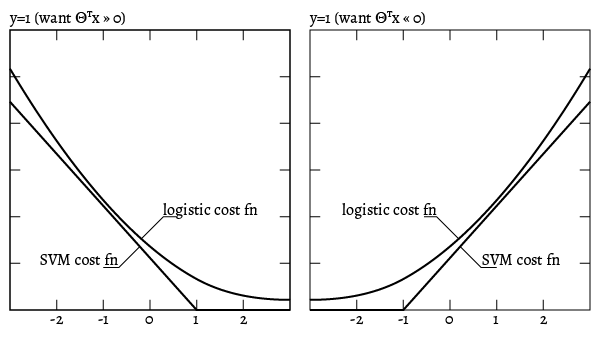
\includegraphics[width=4in]{images/svm-cost-function.png}
\end{center}

Notation: these cost functions are called $\cost_1(z)$ for the $y=1$ case,
and $\cost_0(z)$ for the $y=0$ case.
So a Support Vector Machine has a cost function:

\[ 
    \min_\theta C 
    \sum_{i=1}^m \qty[
        y\s{i} \cost_1(\theta^T x\s{i}) + 
        (1-y\s{i}) \cost_0(\theta^T x\s{i}) 
    ]
    + \frac{1}{2} \sum_{j=0}^n \theta_j^2
\]

By convention, we exclude the factor of $\frac{1}{m}$ from the cost function,
and we use $C$ as the regularization parameter.
That is, we minimize $CA + B$ rather than $A + \lambda B$.
So a small $C$ weighs regularization heavily,
while a large $C$ weighs fitting the training set heavily.
(Think of $C \approx \frac{1}{\lambda}$).

Unlike logistic regression, an SVM does not output a probability.

\[
    \hth(x) = \begin{cases}
        1 \text{ if } \theta^T x \geq 0 \\
        0 \text{ if } \theta^T x < 0
    \end{cases}
\]

\subsection{Large Margin Intuition}

$\cost_1(z)$ is 0 only when $z \geq 1$,
even though we have classified correctly whenever $z \geq 0$.
Likewise, $\cost_0(z)$ is 0 only when $z \leq -1$,
even though we have classified correctly whenever $z < 0$.
Consequently, we want not just to barely get the examples right,
but to have a significant margin of correctness.

Imagine $C$ is extremely large, so we weigh fitting the data very highly.
So whenever $y\s{i} = 1$ we want $\theta^T x \geq 1$,
and whenever $y\s{i} = 0$ we want $\theta^T x \leq -1$.
Since $C$ is so large, we will probably reject any hypothesis which
incorrectly classifies any examples,
so we are left minimizing only the regularization term.

For a linearly separable case, this will draw a decision boundary which
has the largest possible margin between the boundary and the closest points.

For very large $C$, the SVM is very sensitive to outliers,
and might drastically change the boundary to accommodate a single point.
Regularization prevents this.

\subsection{Mathematics behind large margin classification}

Consider $u = \mqty(u_1 \\ u_2)$ and $v = \mqty(v_1 \\ v_2)$.
Then the inner product $u^T v$ is $u_1 v_1 + u_2 v_2$.
And $\norm{u} = \sqrt{u_1^2 + u_2^2}$.
We also have $u^T v = \mathrm{proj}_u(v) \cdot \norm{u} = \mathrm{proj}_v(u) \cdot \norm{v}$.

For the SVM decision boundary, we are effectively minimizing

\[
    \min_\theta \frac{1}{2} \sum_{j=1}^n \theta_j^2  
    \quad \text{ such that } \quad
    \theta^T x\s{i} \geq 1 \text{ if } y\s{i}=1
    \quad \text{ and } \quad
    \theta^T x\s{i} \leq -1 \text{ if } y\s{i}=0
\]

Assume $\theta_0 = 0$.
In the case where $n=2$, we are minimizing $\theta_1^2 + \theta_2^2$,
or equivalently, $\qty(\sqrt{\theta_1^2 + \theta_2^2})^2$, which is $\norm{\theta}^2$.

Now consider $\theta^T x\s{i}$.  This can be thought of as the projection of $x\s{i}$
onto the parameter vector $\theta$ times $\norm{\theta}$.
So we are really finding:

\[
    \min_\theta \frac{1}{2} \norm{\theta}^2
    \quad \text{ such that } \quad
    \mathrm{proj}_\theta x\s{i} \cdot \norm{\theta} \geq 1 \text{ if } y\s{i}=1
    \quad \text{ and } \quad
    \mathrm{proj}_\theta x\s{i} \cdot \norm{\theta} \leq -1 \text{ if } y\s{i}=0
\]

Simplifying notation: let $p\s{i} = \mathrm{proj}_\theta x\s{i}$

This all makes sense if $\theta$ is a vector orthogonal to the decision boundary.
The projections of $x\s{i}$ onto $\theta$ are the distances to the decision boundary,
and we require these all to be above 1.

If the boundary is bad (small margins), then $p\s{i}$ is small,
so by our condition above, $\norm{\theta}$ must be large
(in order for the product to be greater than 1).
Since we're trying to minimize $\norm{\theta}^2$, our algorithm will not choose such a boundary.

Removing the assumption that $\theta_0=0$ just allows us to have 
decision boundaries that do not pass through the origin.
It is just somewhat less obvious to show that this leads to a large margin classifier.

\section{Kernels}

Kernels adapt SVMs to support non-linear models.
One way is to include polynomial features.
This would look like:

\[
    \text{Predict } y=1 \text{ if } \quad
    \theta_0 + \theta_1 x_1 + \theta_2 x_2 + \theta_3 x_1 x_2 + \theta_4 x_1^2 + \dots \geq 0
\]

Instead we can write this more generally as 

\[
    \theta_0 + \theta_1 f_1 + \theta_2 f_2 + \theta_3 f_3 + \theta_4 f_4 + \dots \geq 0
\]

\[
    \theta^T f \geq 0
\]

Where $f$ is the new set of features.  But $f$ doesn't have to come from polynomial features.

Example: compute new features based on proximity to landmark points $l\s{1}, l\s{2}, l\s{3}$.
So $f_j = \text{similarity}\qty(x,l\s{j})$.
We can use a similarity metric like:

\[
    \text{similarity}\qty(x,l\s{j}) = \exp(-\frac{\norm{x-l\s{j}}^2}{2\sigma^2})
\]

The similarity function is called a kernel, and this particular function is called a Gaussian kernel.
It has the feature that $f \approx 1$ when $x \approx l$, and $f \approx 0$ when $x$ is far from $l$.
When $\theta_j$ has a positive value, the classifier will predict 1 for points sufficiently close to
the landmark point $l\s{j}$.

But how do we choose the landmark points $l$?  And what other similarity functions work?

One choice of how to choose $l$ is to use $l\s{i} = x\s{i}$ for $i$ from 1 to $m$.
So you would have as many features as training examples (plus 1 for $\theta_0$),
and the data matrix would become a similarity matrix.
So $X_{ij} = \text{similarity}\qty(x\s{i}, x\s{j})$.

This is a lot of features, but it's way fewer than you would get by adding many polynomial features.

An additional detail: the regularization term $\frac{1}{2} \sum_{i=1}^m \theta_j^2 = \theta^T \theta$
is typically replaced by $\theta^T M \theta$ where $M$ is some matrix that depends on the kernel.
This is done mostly for computational efficiency.

Kernels could be used for other learning methods, but it turns out to be more efficient for SVMs
than for something like logistic regression.

\section{SVM hyperparameters}

Choosing $C$ trades off between bias and variance

Choosing $\sigma^2$ causes features $f_i$ to vary more smoothly,
resulting in higher bias and lower variance.

\section{Using an SVM}

Use a SVM software package to solve for parameters $\theta$

Need to specify $C$ and the kernal.
No kernel is called a ``linear kernel''.  This is okay if $n$ is large, or $m$ is small.
If you choose a Gaussian kernel, you must also specify $\sigma^2$.

You should perform feature scaling before using the Gaussian kernel;
otherwise, larger-valued features will dominate in $\norm{x-l}$.

Any kernel must satisfy a condition called ``Mercer's Theorem''.
A second example is the polynomial kernel:
$k(x,l) = (x^T l + \text{constant})^\text{degree}$,
but this generally performs worse than the Gaussian kernel.
However, sometimes it makes sense for non-negative data.
More rare:

\begin{itemize}
    \item String kernel
    \item Chi-square kernel
    \item Histogram intersection kernel
\end{itemize}

\subsection{Multi-class Classification}

One option is the one-vs-all method
(train $K$ SVMs for $K$ classes, 
get $\theta\s{1}\dots\theta\s{K}$, 
and pick the class with the largest $\theta^T x$).

The other option is just to use the built-in multi-class utility
in the software package you're using.

\subsection{Logistic Regression vs. SVM}

\begin{itemize}
    \item If $n \gg m$
        use logistic regression or a SVM with a linear kernel
    \item If $n$ is small and $m$ is intermediate (10-10,000),
        use a SVM with a Gaussian kernel
    \item If $n$ is small and $m$ is large (50,000+), add more features
        and use logistic regression or an SVM with a linear kernel
\end{itemize}

Neural networks will probably work well for many of these scenarios, 
but may be slower to train.

SVMs have the benefit of convexity, so they will always find a global minimum.
\chapter{Week 8}

\section{Clustering}

A type of unsupervised learning problem in which we identify
distinct groups among our training examples.

\subsection{K-Means Algorithm}

Inputs: the number of clusters $K$ and the data $X$ ($\qty{x\s{1}, \dots, x\s{m}}$).

\begin{enumerate}
    \item Randomly initialize $K$ cluster centroids 
        $\mu_1, \dots, \mu_K$
    \item Cluster assignment step: assign each data point to the closest centroid.
        $c\s{i} :=$ index of closest cluster centroid.
    \item Move centroid step: set each new centroid at the mean value of the data points assigned to it.
    \item Repeat steps 2 and 3 until the centroids no longer move in step 3.
\end{enumerate}

If a centroid ends up with no points assigned to it, you can either re-initialize it,
or drop it (to end up with $K-1$ clusters).

Example for non-separated clusters: t-shirt sizing.

\subsection{Optimization Objective}

Reminder: two sets of variables to keep track of:

$c\s{i} \in \qty{1,2,\dots,K} = $ the index of the cluster to which $x\s{i}$ is assigned.

$\mu_k \in \R^n = $ the centroid of  cluster $k$.

Additional notation: $\mu_{c\s{i}}$ is the centroid of the cluster to which $x\s{i}$ has been assigned.

So now we can write the cost function:

\[
    J\qty(c\s{1}, \dots, c\s{m}, \mu_1, \dots, \mu_K)
    = \frac{1}{m} \sum_{i=1}^m \norm{ x\s{i} - \mu_{c\s{i}} }^2
\]

And we want to find

\[ \min_{c, \mu} J(c, \mu) \]

$J$ is sometimes called the ``Distortion'' of the K-means algorithm.

\subsection{Random Initialization}

One initialization technique is to randomly choose $K$ actual training examples.
This is popular and effective.

If you are unlucky with your initialization, K-means can get stuck in local optima.
This can be resolved by running the entire thing multiple times with different initializations.
Running it 50-1000 times would be pretty typical.
Then pick the clustering that has the lowest distortion $J$.

\subsection{Choosing the number of clusters}

There is not a good way to automate this; doing it by hand is generally accepted as the best.

One ``automatic'' method is the elbow method.
Plot $J$ as a function of $K$, and choose the value for $K$ at which the cost starts going down more slowly.
The problem is, there often is not a clear elbow.

Another choice is to choose pragmatically based on how well it serves some downstream purpose.
If you are selling t-shirts, $K=3$ (small, medium, large) or $K=5$ (add XS and XL) might be good.

\section{Dimensionality Reduction}

Convert data $X$ where $x \in \R^n$
to $Z$ where $z \in \R^k$, and $k<n$.
This helps for compressing data; 100-dimensional data 
takes up much less disk space than 1000-dimensional data.
It also helps for visualization; you cannot visualize 50-dimensional data,
but you can visualize 3 or 2-dimensional data!

\subsection{Principal Component Analysis}

We want to find the $k<n$ vectors $u\s{1}, \dots, u\s{k} \in \R^n$
which minimize the projection error.
By convention, since we just need directions, we will get normalized vectors.

\begin{enumerate}
    \item Perform mean normalization (always) and feature scaling (usually).
        That is, replace each $x\ss{j}{i}$ with $\frac{x_j - \mu_j}{\sigma_j}$.
    \item Compute the covariance matrix
        $\Sigma = \frac{1}{m} X^T X = \frac{1}{m} \sum_{i=1}^n \qty(x\s{i})\qty(x\s{i})^T$
    \item Compute the ``eigenvectors'' (really the singular values) of $\Sigma$:
        \texttt{[U,S,V] = svd(Sigma);}.
        Since $\Sigma$ is symmetric positive-semidefinite, this will give
        the same result as \texttt{eig(Sigma)}, but \texttt{svd} is more numerically stable.
        $Sigma \in \R^{n \times n}$, and $U \in \R^{n \times n}$.
    \item The columns of $U$ are the directions $u$ that we want;
        take the first $k$ columns $U_{\text{reduce}} \in \R^{n \times k}$.
    \item The data $z \in \R^k$ can be found by $z = U_{\text{reduce}}^T x$
\end{enumerate}

\begin{minipage}{0.5\textwidth}
    Implementation:
    \begin{lstlisting}[style=Matlab-editor]
        % Principal Component Analysis
        Sigma = (1/m) * X' * X;
        [U,S,V] = svd(Sigma);
        Ureduce = U(:, 1:k);
      
        Z = X * Ureduce;
        z = Ureduce' * x;
    \end{lstlisting}
\end{minipage}\begin{minipage}{0.5\textwidth}
    Dimensions:
    \begin{itemize}
        \item $X \in \R^{m \times n}$
        \item $\Sigma \in \R^{n \times n}$
        \item $U \in \R^{n \times n}$
        \item $U_{\text{reduce}} \in \R^{n \times k}$
        \item $Z \in \R^{m \times k}$
        \item $x \in \R^n$
        \item $z \in \R^k$
    \end{itemize}
\end{minipage}

\subsection{Reconstruction from Compressed Representation}

Go from $z \in \R^k \to x \in \R^n$
with $x \approx x_{\text{approx}} = U_{\text{reduce}} z$

\subsection{Choosing the Number of Principal Components}

The number $K$ is a parameter of the PCA algorithm.
Given the average squared projection error is given by:

\[ J = \frac{1}{m} \sum_{i=1}^m \norm{ x\s{i} - x_{\text{approx}^{(i)}}}^2 \]

And the total variation in the data is given by:

\[ \frac{1}{m} \sum_{i=1}^m \norm{x\s{i}}^2 \]

We can choose $k$ such that 99\% of variance is retained.
That is, choose the smallest $k$ which satisfies:

\[
    \frac{
        \frac{1}{m} \sum_{i=1}^m \norm{ x\s{i} - x_{\text{approx}^{(i)}}}^2
    }{
        \frac{1}{m} \sum_{i=1}^m \norm{x\s{i}}^2
    }
    \leq 0.01
\]

So really, rather than choosing $k$,
it is more common to choose the amount of variance we want to retain.

One way to satisfy this is to keep increasing $k$
until it no longer satisfies the requirement.
Yikes!

A better way is to examine the diagonal of $S$
(the singular values of the covariance matrix).
The trace of $S$ is the total amount of variance.
Increase $k$ until the first $k$ diagonal entries
over the total is greater than the threshold.

\[ \frac{\sum_{i=1}^k S_{ii}}{\sum_{i=1}^m S_{ii}} \geq 0.99 \]

\subsection{Advice for applying PCA}

Speeding up supervised learning:

Rather than training $X$ against $y$, train $Z$ against $y$.
To make predictions, use $z_{test} = U_{reduce}^T x_{test}$,
and run the model on $z_{test}$.
This should be faster.

Bad use: using PCA to reduce overfitting.
It works okay, but is much less effective than regularization.
PCA does not account for the labels $y$, so when used this way,
it might throw away useful information!

Another bad use: reducing dimension without trying the same problem
on the original data.  If it's not necessary, don't do it!

\chapter{Week 9}

\section{Anomaly Detection}

Given $\qty{x\s{1}, \dots, x\s{m}}$, is $x_{test}$ anomalous?
Flag as an anomaly if $p(x_{test}) < \epsilon$.

Examples: fraud detection, manufacturing, monitoring servers in a data center

\subsection{Gaussian Distribution}

Say $x \in \R$.  If $x$ has a Gaussian distribution with mean $\mu$
and variance $\sigma^2$, then we say $x \sim N(\mu,\sigma^2)$.

\[ 
    p(x; \mu, \sigma^2) = 
    \frac{1}{\sqrt{2\pi} \sigma} 
    \exp(-\frac{(x-\mu)^2}{2\sigma^2}) 
\]

Given a dataset, find $\mu$ and $\sigma^2$:

\[
    \mu \approx \bar{x} = \frac{1}{m} \sum_{i=1}^m x\s{i}
    \quad
    \sigma^2 \approx s = \frac{1}{m} \sum_{i=1}^m \qty(x\s{i}-\mu)^2
\]

(really the coefficient should be $\frac{1}{m-1}$ in the latter formula,
but for large $m$ it makes little difference)

\subsection{Anomaly Detection Algorithm}

Given a data set $\qty{x\s{1}, \dots, x\s{m}}$ where each $x \in \R^n$,

\[
    p(x)
    = p(x_1; \mu_1, \sigma_1^2)
      p(x_2; \mu_2, \sigma_2^2) \dots 
      p(x_n; \mu_n, \sigma_n^2)
    = \prod_{j=1}^n p(x_j; \mu_j, \sigma_j^2)
\]

We assume $x_j \sim N(\mu_j, \sigma_j^2)$,
and that all $x_j$ are independent.
They are almost definitely not independent, but the algorithm works okay anyway.

Algorithm:
\begin{enumerate}
    \item Choose features $x_i \in \R^n$
    \item Fit parameters $\mu_1, \dots, \mu_n, \sigma_1^2, \dots, \sigma_n^2$
        using maximum likelihood estimators
    \item Given a new example $x$, compute $p(x)$ using the product above
    \item Classify as anomalous if $p(x) < \epsilon$
\end{enumerate}

Since we are just using the value of the probability density function,
this doesn't have a whole lot of meaning.
But it works.

\subsection{Anomaly Detection System}

In order to evaluate the algorithm (for choosing features, etc.),
we want a real-valued metric.
Assume we have labeled data, with $y=1$ indicating an anomaly.
Assume the training set is ``normal''.
Assume also that the cross-validation and tests sets have some normal data and some anomalies.
Ensure that the anomalies are split between the cross-validation and test sets.

Possible evaluation metrics:
\begin{itemize}
    \item True positive, false positive, false negative, true negative
    \item Precision/Recall
    \item $F_1$-score
\end{itemize}

You can choose $\epsilon$ to maximize your metric on the cross-validation set.
This should be monotonic, so a binary search should work well.

\subsection{Anomaly Detection vs. Supervised Learning}

If we have labeled data, why not just use supervised learning?

Anomaly detection:
\begin{itemize}
    \item Very small number of positive Examples
    \item Large number of negative example
    \item Many different ``types'' of anomalies; maybe future examples
        would be different from ones we've already seen
\end{itemize}

Supervised learning:
\begin{itemize}
    \item Large number of positive and negative examples
    \item Enough positive examples for the algorithm to get a sense of what
        positive examples are like in general
\end{itemize}

\subsection{Choosing What Features to Use}

Plot histograms to check if a feature is at least vaguely gaussian,
or can be transformed to be gaussian.

Example transformations:
\begin{itemize}
    \item $x \to \log(x+c)$
    \item $x \to x^{1/c}$
\end{itemize}

Error analysis: run the algorithm;
examine the incorrect classifications;
use that examination as inspiration to develop new features.

In particular, choose features that might take on unusually large values
if something unusual is going on.

\subsection{The Multivariate Gaussian Distribution}

This has some advantages relative to the version with the independence assumption,
and some disadvantages.
In particular, it handles colinear features much better by accounting for covariance.

Parameters: a mean vector $\mu \in \R^n$,
and a covariance matrix $\Sigma \in \R^{n\times n}$.

\[
    p(x; \mu, \Sigma)
    = \frac{1}{ (2\pi)^{n/2} \det(\Sigma)^{1/2}}
      \exp( -\frac{1}{2} (x-\mu)^T \Sigma^{-1} (x-\mu))
\]

where

\[
    \mu = \frac{1}{m} \sum_{i=1}^m x\s{i}
    \quad
    \Sigma = \frac{1}{m} \sum_{i=1}^m (x\s{i} - \mu)(x\s{i} - \mu)^T
\]

This is the same as the original model, given the constraint that $\Sigma$ is diagonal.

Disadvantaves of the multivariate model:
computationally more expensive than the original model,
and does not scale as well to large $n$ (because of the matrix inverse).
Furthermore, for the multivariate model you must have $m>n$ (ideally $m>10n$)---
otherwise $\Sigma$ is not invertible, where the original model has no such constraint.

\section{Recommender Systems}

Consider a set of users who watched a set of movies:

\begin{center}
\begin{tabular}{l|cccc}
    Movie                & Alice (1) & Bob (2) & Carol (3) & Dave (4) \\ \hline
    Love at Last         & 5 & 5 & 0 & 0 \\
    Romance Forever      & 5 & - & - & 0 \\
    Cute Puppies of Love & - & 4 & 0 & - \\
    Nonstop Car Chases   & 0 & 0 & 5 & 4 \\
    Swords vs. Karate    & 0 & 0 & 5 & -
\end{tabular}
\end{center}

So Alice and Bob appear to like romance, while Carol and Dave like action.

Notation:
\begin{itemize}
    \item $n_u=$ number of users
    \item $n_m=$ number of movies
    \item $r(i,j)=$ 1 if user $j$ has rated movie $i$
    \item $y\s{i,j}=$ rating given by user $j$ to movie $i$
\end{itemize}

Given this incomplete dataset, predict the missing values.

\subsection{Content-based Recommendation}

Suppose you have a set of $n$ features describing each movie in addition to the ratings:

\begin{center}
\begin{tabular}{l|cccc|cc}
    Movie                & Alice (1) & Bob (2) & Carol (3) & Dave (4) & $x_1$ & $x_2$ \\ \hline
    Love at Last         & 5 & 5 & 0 & 0 & 0.90 & 0.00 \\
    Romance Forever      & 5 & - & - & 0 & 1.00 & 0.01 \\
    Cute Puppies of Love & - & 4 & 0 & - & 0.99 & 0.00 \\
    Nonstop Car Chases   & 0 & 0 & 5 & 4 & 0.10 & 1.00 \\
    Swords vs. Karate    & 0 & 0 & 5 & - & 0.00 & 0.90
\end{tabular}
\end{center}

One option is to treat predicting ratings for each user as a separate linear regression problem.
For each user $j$, learn a set of parameters $\theta\s{j} \in \R^{n+1}$.
Predict user $j$ as rating movie $i$ with $(\theta\s{j})^T x\s{i}$ stars.

In other words, (with $m\s{j}=$ number of movies rated by person $j$), we learn $\theta\s{j}$ with:

\[
    \min_{\theta\s{j}}
    \frac{1}{2} \sum_{i:r(i,j)=1} \qty( (\theta\s{j})^T x\s{i} - y\s{i,j} )^2
    + \frac{\lambda}{2} \sum_{k=1}^n \qty( \theta\ss{k}{j} )^2
\]

And to learn all of $\theta\s{1}, \dots, \theta\s{n_u}$ we apply a simple variation
where our total cost includes the cost for each user:

\[
    \min_{\theta\s{1}, \dots, \theta\s{n_u}}
    \frac{1}{2} \sum_{j=1}^{n_u} \sum_{i:r(i,j)=1} \qty( (\theta\s{j})^T x\s{i} - y\s{i,j} )^2
    + \frac{\lambda}{2} \sum_{j=1}^{n_u} \sum_{k=1}^n \qty( \theta\ss{k}{j} )^2
\]

The gradient descent update for this looks like:

\[
    \theta\ss{k}{j} := \theta\ss{k}{j} - \alpha \qty(
        \sum_{i:r(i,j)=1} \qty( 
            (\theta\s{j})^T x\s{i} - y\s{i,j} 
        ) x\ss{k}{i}
        + \lambda \theta\ss{k}{j}
    )
\]

(where $\theta_0=0$ so we do not regularize the constant term)

\subsection{Collaborative Filtering}

The previous example assumed that you are provided with $x_1$ (romance) and $x_2$ (action).
Now, assume instead that each user ($i$) has rated their own enjoyment of romance and action movies ($\theta\s{i}$)

\[
    \theta\s{1} = \mqty(0\\5\\0) \quad
    \theta\s{2} = \mqty(0\\5\\0) \quad
    \theta\s{3} = \mqty(0\\0\\5) \quad
    \theta\s{4} = \mqty(0\\0\\5)
\]

So again, Alice and Bob enjoy romance while Carol and Dave enjoy action.
From here, it is possible to infer the values of $x_1$ and $x_2$ for a given movie $x\s{i}$:

\[
    \text{Find } x\s{1} \text{ such that } \qty(\theta\s{1})^T x\s{1} \approx 5
\]

More formally, given $\theta\s{1}, \dots, \theta\s{n_u}$ to learn $x\s{i}$:

\[
    \min_{x\s{i}}
    \frac{1}{2} \sum_{ j:r(i,j)=1 } \qty(
        \qty(\theta\s{j})^T x\s{i} - y\s{i,j}
    )^2 +
    \frac{\lambda}{2} \sum_{k=1}^n \qty( x\ss{k}{i} )^2
\]

So we minimize the sum over all users $j$ that have rated movie $i$
of the squared error from the actual rating $y\s{i,j}$.

More generally, given $\theta\s{1}, \dots, \theta\s{n_u}$ to learn $x\s{1}, \dots, x\s{n_m}$:

\[
    \min_{x\s{i}}
    \frac{1}{2} \sum_{i=1}^{n_m} \sum_{ j:r(i,j)=1 } \qty(
        \qty(\theta\s{j})^T x\s{i} - y\s{i,j}
    )^2 +
    \frac{\lambda}{2} \sum_{i=1}^{n_m} \sum_{k=1}^n \qty( x\ss{k}{i} )^2
\]

This is a simple change: both terms in the cost now sum over all movies.

We can make predicitons in both directions:
given $x\s{1}, \dots, x\s{n_m}$ we can estimate $\theta\s{1}, \dots, \theta\s{n_u}$,
and likewise given $\theta\s{1}, \dots, \theta\s{n_u}$ we can estimate $x\s{1}, \dots, x\s{n_m}$.
Now, we can take an iterative approach.  Given an initial guess $\theta$, can can predict:

\[ \theta \to x \to \theta \to x \to \theta \to x \to \dots \]

And this actually works, but it is not yet ideal.

\subsection{Collaborative Filtering Algorithm}

Instead of alternating between predicting $\theta$ and $x$, we can throw them into the same objective function.

\[
    J\qty( x\s{1}, \dots, x\s{n_m}, \theta\s{1}, \dots, \theta\s{n_u} ) = 
    \frac{1}{s} \sum_{(i,j) : r(i,j) = 1} \qty(
        (\theta\s{j})^T x\s{i} - y\s{i,j}
    )^2 +
    \frac{\lambda}{2} \sum_{i=1}^{n_m} \sum_{k=1}^n \qty( x\ss{k}{i} )^2 + 
    \frac{\lambda}{2} \sum_{j=1}^{n_u} \sum_{k=1}^n \qty( \theta\ss{k}{i} )^2
\]

And now, we minimize $J$ over all $x$ and $\theta$.
If you hold $x$ constant then you are solving the first problem where we were given features for each movie.
If you hold $\theta$ constant then you are solving the second problem where we were given parameters for each user.

By convention, in this case, we will dispense with the constant terms, so $x,\theta \in \R^n$.
If the algorithm wants a constant feature, it can learn one.

The gradient will have terms for both $x$ and $\theta$.

For this recommendation algorithm, initialize $x$ and $\theta$ to small random values
to break symmetry and ensure that the algorithm learns $x\s{i}$ that are different from one another.

Our gradient descent steps will look like this:

\[
    x\ss{k}{i} := x\ss{k}{i} - \alpha \qty(
        \sum_{j:r(i,j)=1} \qty((\theta\s{j})^T x\s{i} - y\s{i,j}) \theta\ss{k}{j} 
        + \lambda x\ss{k}{i}
    )
\]

\[
    \theta\ss{k}{i} := x\ss{k}{i} - \alpha \qty(
        \sum_{j:r(i,j)=1} \qty((\theta\s{j})^T x\s{i} - y\s{i,j}) x\ss{k}{j} 
        + \lambda \theta\ss{k}{i}
    )
\]

Where the terms in parentheses are $\pdv{x\ss{k}{i}} J(x,\theta)$ and $\pdv{\theta\ss{k}{i}} J(x,\theta)$

For a user $j$ with parameters $\theta$ and a movie $i$ with features $x$, predict a rating of $\theta^T x$
(assuming $r(i,j)=0$, otherwise we already know the answer!).

\chapter{Week 10}

\section{Gradient Descent with Large Datasets}

One way to build a strong classifier is to train a low-bias learning algorithm and train 
it on a large amount of data.
But gradient descent typically involves summation over $m$ entries, so when $m$ is very
large, this becomes computationally very expensive.
Sanity check: you can also start by training on a subset of the data.
Learning curves ($J$ vs $m$) can tell you whether training on the full data will improve performance.

\subsection{Stochastic Gradient Descent}

Batch Gradient Descent: each update uses all $m$ training examples.
Using linear regression as the example:

\[
    \hth(x\s{i}) = \theta^T x
    \qquad
    J(\theta) = \frac{1}{2m} \sum_{i=1}^m (\hth(x\s{i}) - y\s{i})^2
    \qquad
    \theta_j := \theta_j - \alpha \frac{1}{m} \sum_{i=1}^m (\hth(x\s{i}) - y\s{i})x\ss{j}{i}
\]

Now, write the cost for an individual data point:

\[
    \cost(\theta, (x\s{i}, y\s{i})) = \frac{1}{2}\qty( \hth(x\s{i}) - y\s{i} )^2
    \qquad
    J(\theta) = \frac{1}{m} \sum_{i=1}^m \cost(\theta, (x\s{i}, y\s{i}))
    \qquad
    \pdv{\theta_j} \cost(\theta, x, y) = (\hth(x) - u) x
\]

For Stochastic Gradient Descent:

\begin{enumerate}
    \item Randomly shuffle the dataset (just in case there is an ordering)
    \item Repeat:
    \begin{enumerate}
        \item for $i \in {1, \dots, m}$:
        \begin{enumerate}
            \item $\theta_j = \pdv{\theta_j}\cost(\theta, x\s{i}, y\s{i})$
                  for $j \in {1, \dots, n}$
        \end{enumerate}
    \end{enumerate}
\end{enumerate}

In other words, compute the gradient for the first data point, and update $\theta$.
Then compute the gradient for the second data point, and update $\theta$, and so on.
Stochastic gradient descent does not take as direct a path toward the global minimum;
it tends to wander.
But each update is much faster.

\subsection{Mini-Batch Gradient Descent}

Mini-batch gradient descent falls in between the batch and stochastic algorithms.
Rather than using all $m$ examples or only 1 example per update, we will use $b$
examples, with $1<b<m$.
Typical values for $b$ range from 2--100.
We still shuffle the dataset, and use $b$ examples at a time, going through the entire data set.

This can perform better than stochastic gradient descent, because good vectorization can
make the summations run more efficiently.

\subsection{Convergence}

For batch gradient descent, we can verify it is working by
ensuring that $J$ decreases on each iteration.

For stochastic gradient descent, we can do the same verification by ensuring that
the cost for the training example is lower after the update compared to before.
Plotting $\cost(\theta, x, y)$ averaged over the last 1000 (or so) examples should show a
plot that generally appears to converge.
Changing this number can make the trend more apparent.
If the plot appears to diverge, use a smaller $\alpha$.

If we want $\theta$ to be more certain to converge, you can decrease $\alpha$ over time:

\[ \alpha = \frac{\text{const1}}{\text{iterationNumber} + \text{const2}} \]

But this is often not done because fiddling with the constants takes time.

\section{Online Learning}

Online learning handles the scenario where there is a continuous stream of data coming in which
should refine the algorithm's predictions.

\begin{enumerate}
    \item Repeat forever:
    \begin{enumerate}
        \item Get $(x,y)$ corresponding to a single new data point
        \item Update $\theta$ using $(x,y)$
        \begin{enumerate}
            \item $\theta_j := \theta_j - \alpha (\hth(x) - y)x \forall j \in {1,\dots,n}$
        \end{enumerate}
    \end{enumerate}
\end{enumerate}

In this case, there is no fixed training set - just one example at a time.
If the nature of the data changes over time, the algorithm will adapt.

This applies well to predicted click-through-rates, showing special offers on websites, etc.

\section{Map Reduce and Data Parallelism}

Each machine, in parallel, trains on a fraction of the data to compute a gradient descent update.
Each calculates its own value for the gradient, and then they are averaged on a master machine.
If there were no network latency, this could speed up processing by as much as $N$ times,
where $N$ is the number of machines.
Whenever the bulk of a learning algorithm can be expressed as a sum over a large data set,
then map-reduce can be a good way to speed up the work.

Exploiting multiple cores on a single machine can yield similar benefits.
Some numerical linear algebra libraries will do this automatically.
% \chapter{Week 11}

\section{Case Study: Photo OCR}

\subsection{Problem Description and Pipeline}

OCR stands for Optical Character Recognition.
There are two steps: first, identifying where there is text in a picture,
then segmenting that text into characters,
and finally identifying the characters in that text.
This is not difficult for scanned documents, but is very difficult for photographs.

This sequence of steps, each of which uses ML, is an example of a pipeline.

\subsection{Sliding Windows}

Pedestrian detection is a simpler problem, because the aspect ratios of rectangles
around a person all have about the same size.
A neural network can be trained to take a window and identify whether or not it
includes a pedestrian.
Then the window is shifted, and the classification is repeated.
This entire process can be repeated with a variety of window sizes.

For an example like text detection, wherein the aspect ratios vary, we can still
use windows of a fixed size, but then apply an ``expansion operator'' to attempt
to combine adjacent regions of text.

Sliding windows can also be used for character segmentation; in this case, a neural
network can be trained to identify whether a window contains the midpoint between
two characters.

\subsection{Getting Lots of Data and Artificial Data}

For character recognition, you can use free font data to generate artificial data
to combine with real data.
You can also take real data and apply transformations (like distortion) to amplify the data set.
This technique works quite well for generating speech recognition sample data as well.
The distortions should be meaningful and representative of what might appear in the test set.

Before expanding the data set, make sure you have a low-bias classifier or it will not help!

``How much work would it be to get 10 times as much data as we currently have?''

\begin{itemize}
    \item Artificial data synthesis
    \item Collect and label it yourself
    \item ``Crowd source'' (Amazon Mechanical Turk)
\end{itemize}

\subsection{Ceiling Analysis: What Part of the Pipeline to Work on Next}

Having a single real-valued metric helps us to decide what to work on.

Ceiling analysis: given perfect inputs for each stage in the pipeline,
what is the impact on the overall system accuracy?
Whichever stage provides the largest jump is probably a good place to spend effort.
If having perfect text location data makes the overall system much better, spend time
on text identification!


\end{document}